\documentclass[a4paper,12pt]{report}

\usepackage[utf8]{inputenc}
\usepackage{fontspec}
\usepackage{graphicx}
\usepackage{wrapfig}
\usepackage{setspace}
\usepackage[titletoc]{appendix}
\usepackage{pdfpages} 
\usepackage{url}

\setlength{\parindent}{0em}
\setlength{\parskip}{1em}

\setmainfont[
BoldFont=arialbd.ttf,
ItalicFont=ariali.ttf,
BoldItalicFont=arialbi.ttf
]{arial.ttf}

\author{Arundathi Shaji Shanthini}

\renewcommand{\bibname}{References}

%\setlength{\voffset}{-0.75in}

\begin{document}
%%%%%%%%%%%COVERSHEET%%%%%%%%%%%%%%%%%
\begin{titlepage}
    \setlength{\voffset}{-1.8in}
    \noindent \noindent \makebox[\textwidth]{
\includegraphics[width=1.55\textwidth]{images/Coversheet_Header_black_with_text.png}}
    
    \vspace{30mm}

    \begin{center}
        {\LARGE \textbf{BEng Project}}\\
        \vspace{4mm}
        {\Huge \textbf{Interim Report}}
    \end{center}
    
    \vspace{10mm}
    
    \begin{center}
    \begin{spacing}{1.8}
    {\LARGE
   Dynamic Modelling of a Continuum Robotic Snake-arm and its Performance Evaluation by Analysing Robustness}
    \end{spacing}
    \end{center}
    
    \vspace{18mm}
    
     \begin{tabular}{ll}
        \textbf{Student Name:}  & \hspace{4mm} Arundathi Shaji Shanthini \\
       \textbf{Contact e-mail:} & \hspace{4mm} arundathi.shanthini.16@ucl.ac.uk \\
        \textbf{Student number:} & \hspace{4mm} 16018351 \\ \\ 
        \textbf{Project Supervisor:}  & \hspace{4mm} Prof. Sarah Spurgeon \\
        \textbf{Contact e-mail:}  & \hspace{4mm} s.spurgeon@ucl.ac.uk \\
         \textbf{Department:} & \hspace{4mm} Department of Electronic and Electrical Engineering\\ \\ 
          \textbf{Submission Date:} & \hspace{4mm} 13\textsuperscript{th} of December 2019
    \end{tabular}
\end{titlepage}
%%%%%%%%%%%%%%%%%%%%%%%%%%%%%%%%%%%%%%

\pagebreak

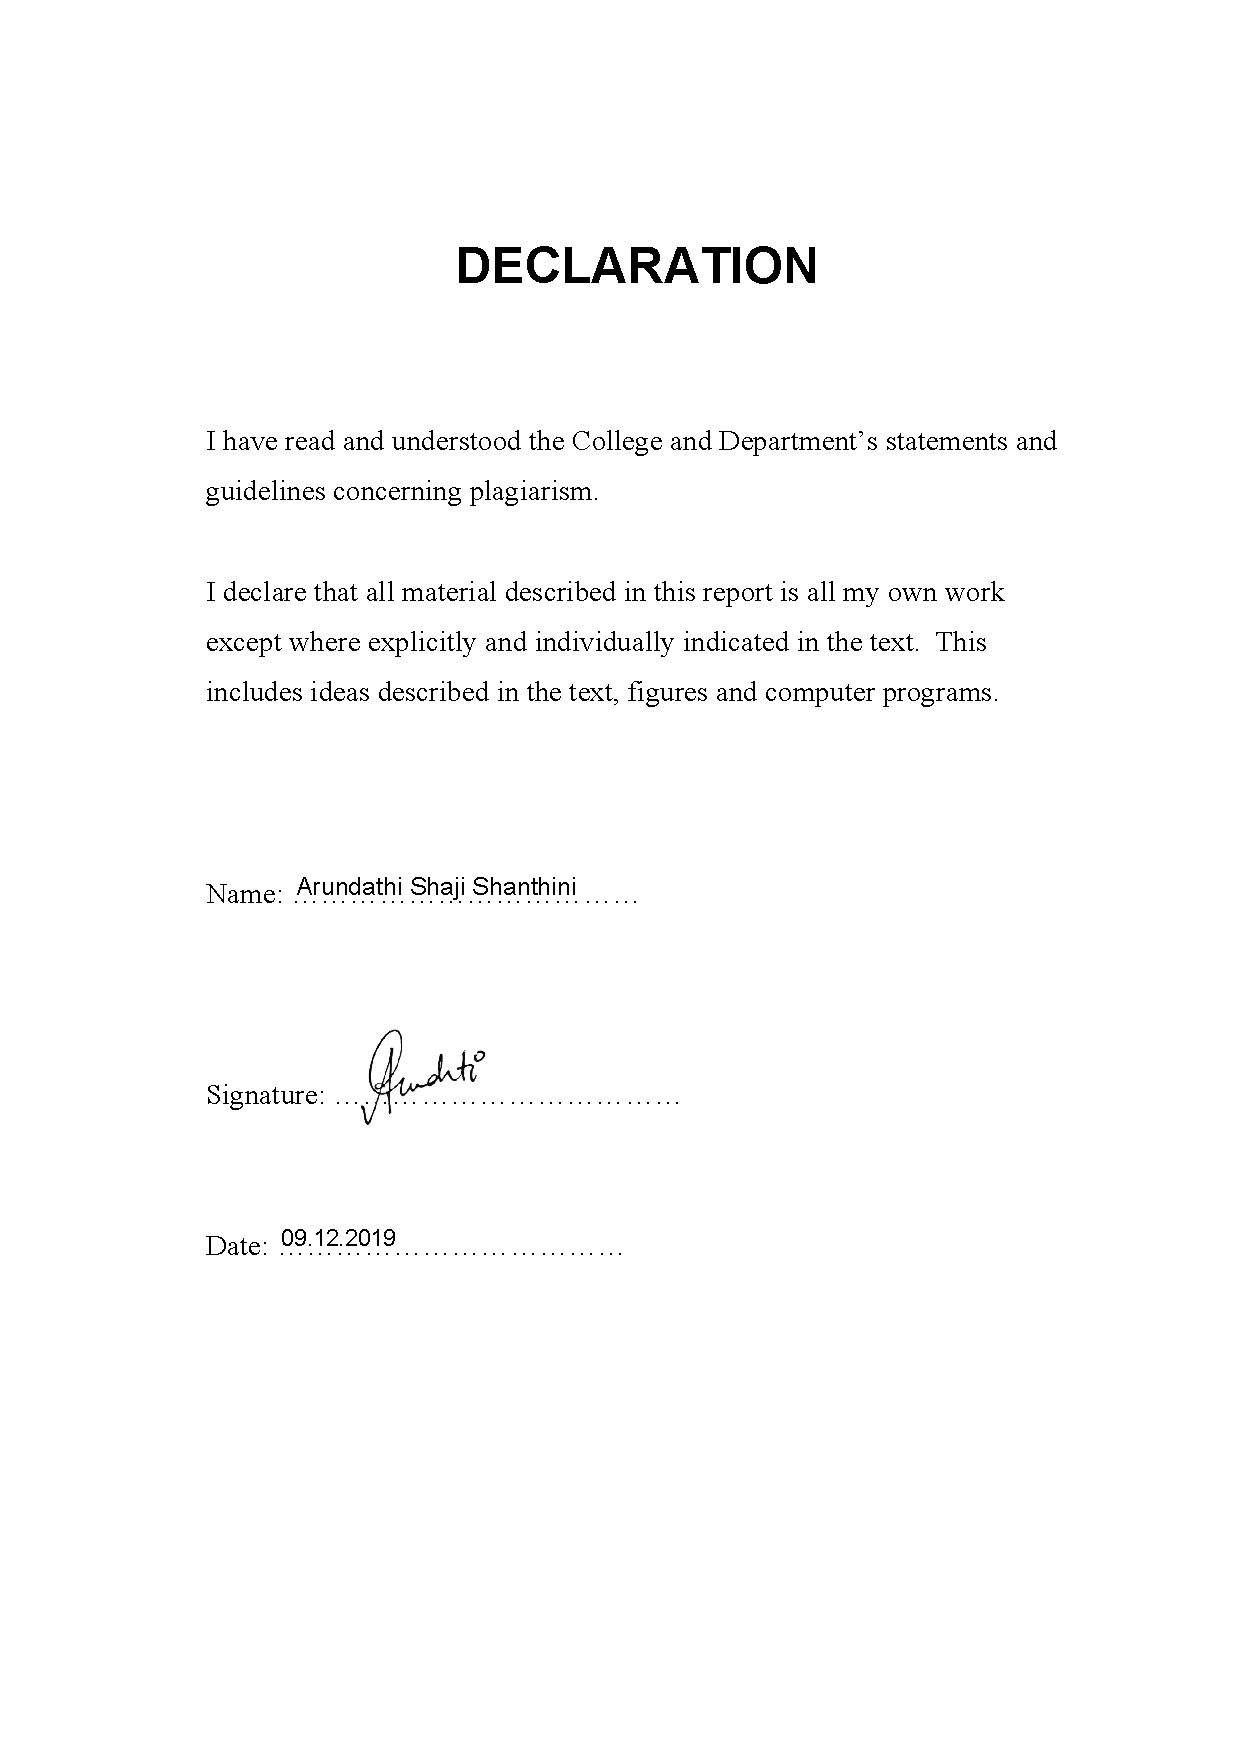
\includepdf[page=-]{files/Declaration}

\tableofcontents

\pagebreak

%%%%%%%%%%% ABSTRACT %%%%%%%%%%%%%%%%%
\begin{abstract}
    \ldots
    
\end{abstract}
%%%%%%%%%%%%%%%%%%%%%%%%%%%%%%%%%%%%%%

%%%%%%%%%%% INTRODUCTION %%%%%%%%%%%%%%%%%
\chapter{Introduction}
\section{Project Description and Motivations}
Industrial robots over the years are being developed from being just pick and place robotic arms to systems with better intelligence, accessibility and manoeuvrability properties that can perform a myriad of operations. Specially over the past decade, there has also been a lot of interest towards bio-mimetic or bio-inspired robotic systems that involves studying concepts from nature  

%\begin{wrapfigure}{l}{0.25\textwidth}
%	\centering
%	\includegraphics[width=0.25\textwidth]{contour}
%	\caption{}
%\end{wrapfigure}
(Advantages if this robot):
- can access remote areas (slender or heavier payload)
- has no electronics in the robot itself makes it access hazardous environments with no issues (easy risk assessment) benign 
- high data quality 

\section{Aims and Objectives}
The aim of the project is to contribute to the modelling and control effort around the snake-arm at Here East by developing and implementing a mathematical model and testing a control system configuration suitable for the task.
For this the first objective would be to develop a model that best represents the system. This model will then be implemented in Simulink and will be tested to ensure that the behaviour is as expected and represents the physical snake-arm well. 
The next objective is to define control requirements for the automation of the optical metrology process and design control strategies that performs the operation with the required accuracy. Through iterative testing, the model will be improved over the course of the project till satisfactory results are obtained.
Finally, the project also aims to investigate the robustness of the system since it is expected to work in environments with varied conditions where external disturbances affecting the arm’s propagation might be considerable. It is also expected that depending on the technique adopted for the optical metrology different payloads may be attached to the head of the snakebot. The payload may also change in mass especially in occasions when improvements have been made to the same metrology technique under consideration. Therefore, the robustness of the system under the influence of change of mass of the head and the external disturbances will be investigated through experiments in the simulation software.
The summary of the main objectives of the project as mentioned above are:
\begin{itemize}
	\item Develop and implement a mathematical model that best represents the snake-arm at Here East.
	\item Design and test control strategies that will help control the path followed by the arm during the metrology task.
	\item Analyse the robustness of the control system configuration developed by running experiments with varied physical parameters.
\end{itemize}
 
\section{Literature Review}
This section discusses the primary sources identified from the literature explored for this project.
Since, the system under consideration is specifically that of the OC Robotics snake arm, material published by the founders Graham A. and Buckingham R. were of immense interest. Even though material directly related to the robot or its technology could not be found, [1-3] by these authors were a good introduction to their work on snake arms and the bigger context of the  varied applications of such robots. The slides in [3], also discussed the main features of  snake arm robots.
Given that the system was identified as a wire rope driven, hollow core structure with passive revolute joints connecting the links to each other, attempts were made to identify literature around modelling of a similar system. The work of Jones B. et al. [4] (dated 2006) has been cited in most papers. His work on kinematics for multi-section continuum robots seems to be the inspiration for most of the work around continuum snake arm robots. The works of Li Z. et al. [5-10] discusses how the skeleton of the robot is inspired from the skeleton of a snake and the idea of a the cable driven structure is inspired from the muscle arrangement in the tentacle of an octopus. Even though across various papers their work discusses the kinematic model of the snake arm robot, they do not discuss much about the dynamic model and control of the system. The references [11-14] represents the OC robotics snake arm the most. The system described by these papers uses a cable-driven snake arm in which the cables are controlled at the base with maxon motors exactly like the snake arm at Here East. The papers published by Tang L. et al. [11, 12] describes the design, motion planning and path tracking of the snake-arm. The work of Tang J. et al. [13] describes the design of this hyper-redundant manipulator. However, the work of Xu W. et al [14] dated 2018, remains the most suitable reference found so far as it discusses the dynamic model and control of the cable-driven snake arm in great detail. 

\cite{singh2014continuum} this discusses the idea of continuum robots 


%%%%%%%%%%%%%%%%%%%%%%%%%%%%%%%%%%%%%%

%%%%%%%%%%% MATHEMATICAL MODELLING %%%%%%%%%%%%%%%%%
\chapter{Mathematical Modelling}
\section{Project Scheduling}
\section{Understanding the system}
To find the most suitable mathematical model that suits the snake-arm, a clear understanding of the system itself was to be established. Understanding the actuators that drive the system and understanding what parameters can be controlled was also essential to determine what terms should be used to represent the mathematical model.

The videos that have been made available by OC Robotics specially [15, 16], helped understand the snake-arm and its capabilities to an extent. In the video for Maxon Motors [16], Graham A. talks about the unique nose following property of the snake arm robot and how it is easily controlled using a proprietary software. The robot is driven by the wire ropes [17] that run in parallel on the surface outside the link (as can be seen in the picture on the top-right of Fig 1) casing and the cables are controlled 30 or more motors [16] in the base (as can be seen in the picture on the left and bottom-right of Fig. 1) using maxon motors as it offers higher power density. The nose of the snake arm can accommodate different payloads and the snake arm also has a hollow core thus allowing cables, hoses or any other equipment required by the specific payload to be routed through the centre of the snake arm.

From these information, currently work of Xu, W et. al. [14] looks like the most suitable model. 

\section{Kinematic Modelling}
\section{Dynamic Modelling}
THe following have been identified to help with the dynamics
\cite{mu_liu_xu_lou_liang_2019} 
\section{Progress to Date}
%%%%%%%%%%%%%%%%%%%%%%%%%%%%%%%%%%%%%%

%%%%%%%%%%% MATHEMATICAL MODELLING %%%%%%%%%%%%%%%%%
\chapter{Initial Simulation Results}
\section{Project Scheduling}
 
%%%%%%%%%%%%%%%%%%%%%%%%%%%%%%%%%%%%%%

%%%%%%%%%%% CONCLUSIONS %%%%%%%%%%%%%%%%%
\chapter{Summary of Difficulties and Issues}
\section{List of Difficulties ans Issues}
\begin{itemize}
	\item Preparatory phase took longer than expected  
\end{itemize}
\section{Failure Risk Assessment}
The project mainly involves modelling of a dynamic system and analysing its behaviour under control system configurations. Therefore, with respect to this project, failure can be mainly thought of as not being able to simulate the behaviour of the real dynamic system using the mathematical model chosen or not being able to obtain expected tracking of the reference parameters.
Several factors can cause these failures, therefore to tackle such unexpected behaviour and/or arbitrary results, an iterative method is used for testing and improvement of the results. From a very early stage (as can be seen in the Gantt Chart), the results will be compiled, understood and analysed to understand how improvements can be made. Necessary changes will be then incorporated, and this process will be repeated till desired tracking of parameters is achieved. Each iteration may involve improvements made through educated trial and error methods and/or experiments. 
Iterations may also involve major changes to the simulation model. If after several attempts desired results could not be obtained, then different control system configurations will be attempted and changes supporting improved results will be adopted. The mathematical model representing the snake-arm may also be replaced to use simpler or more complex. To make it easier if the mathematical model fails to behave as expected, during literature review possible variations of the mathematical model will be noted and recorded.
Currently, the robotic snake-arm has been identified as a continuum robot however, if this approach fails to represent the behaviour of the model, then an alternative model that represents the system will be identified or else the last resort would be fall back on the simplified option for the mathematical model which is the approach of a simplifying the snake-arm as a modular robotic arm with several rigid links of a fixed length. The modular “vertebrae-like” model would still simulate the behaviour of the arm even though the number of degrees of freedom of the system might reduce significantly.
Additionally, the weekly project tutorials with the project supervisor will also help give new perspectives and ideas on how the results can be improved.

\section{Safety Risk Assessment}
Since the project does not include any tasks involving hardware or use of laboratory equipment and machinery, the risks associated are only those around working on a computer. Some of the main safety risks associated to working on a computer have been identified as:
\begin{itemize}
	\item  	\textbf{Eyestrain:}  Long hours of looking into a screen especially with incorrect screen settings and in a room with poor/intrusive lighting conditions can lead to eyestrain and headache related to it. \\ \\
	\textbf{Control measures:}
	\begin{itemize}
		\item Ensure that the screen settings are suitable for the lighting conditions of the room. The contrast, brightness and colours of the screen must be easy on the eyes.
		\item Face your screen away from intrusive light or glare. This can be avoided by facing it away from windows, bulbs and bright light in the room.
		\item Ensure that the screen is clean.
		\item Make sure that while reading, the screen in zoomed in sufficiently so that the letters are large enough to be read from a comfortable position.
		\item Ensure that the text on the screen is sharp and in focus. The screen shouldn’t flicker, and the text must not appear to be moving.
		\item Give your eyes a break from looking into the screen by looking into the distance from time to time.
	\end{itemize}
	\item \textbf{Poor Posture:} Poor posture while sitting at a work station can lead to discomfort from aches, backpain etc. and may even cause injury. Poor posture may even be caused due to poor workstation set up.\\ \\
	\textbf{Control measures:}
	\begin{itemize}
		\item Ensure that you are sitting upright with your back positioned comfortably on the backrest of the chair. Sit close to the desk to prevent leaning forward uncomfortably.
		\item Ensure that your eyes are at the same height as the top of the screen.
		\item Take short and frequent breaks and change position if possible.
	\end{itemize}
	\item \textbf{Repetitive movements:} Poorly designed workstations or uncomfortable working postures might lead to repetitive strained movements and can cause repetitive strain injuries. \\ \\
	\textbf{Control measures:}
	\begin{itemize}
		\item Take short and frequent breaks and if possible, stretch and change position.
		\item Make sure there is space under the desk to move legs.
		\item Ensure that the workstation layout does not contribute to repetitive strained movements. Choose a comfortable space.
		\item Position the mouse such that it is within easy reach and can be held with a straight wrist
		\item When not typing use the space in front of keyboard to rest your wrists and hands.
		\item Do not overstrain muscles by overstretching fingers when typing or holding onto the mouse with a tight grip.
		\item Sit upright and close to the desk to reduce working with the mouse with your arm stretched.
	\end{itemize}
	\item \textbf{Tripping:} When working in computer labs or study spaces there is a risk of tripping over objects or slipping on spillages. \\ \\
	\textbf{Control measures:}
	\begin{itemize}
		\item Be mindful and careful of obstructions on the floor/walkways even in rooms that you are used to working in. Avoid walking around carelessly or looking into the screen of the computer.
		\item Inform the responsible management if any major obstruction with potential risk is noticed. This may include damaged floors, trailing cables, inadequate housekeeping, incorrect lighting levels etc.
	\end{itemize}
	\item 	\textbf{Poor lighting conditions:} Poor lighting conditions refers to both insufficient lighting as well as excessive lighting of a room. Poor lighting conditions may cause headaches or sore eyes.\\ \\
	\textbf{Control measures:}
	\begin{itemize}
		\item Control the lighting in the room suitably.
		\item Adjust the blinds to control natural light levels or to avoid glare on screens.
	\end{itemize}
	\item \textbf{Lone working:} When working alone in the office there is risk of injuries, emergencies etc. with inadequate provision for help.\\ \\
	\textbf{Control measures:}
	\begin{itemize}
		\item Avoid non-routine working.
		\item Be aware of the risks and precaution associated to the work undertaken.
		\item Have the information and knowledge of how to deal with emergencies
	\end{itemize}
\end{itemize}

The above-mentioned risks are the main risks associated to working on a computer. A more exhaustive list of risks, including ones that are very unlikely, were submitted via RiskNET. The approved risk assessment report can be found in Appendix \ref{appendix:b}.	


\section{Additional Work to Complete Goals}
%%%%%%%%%%%%%%%%%%%%%%%%%%%%%%%%%%%%%%

%%%%%%%%%%% APPENDIX %%%%%%%%%%%%%%%%%
\begin{appendices}
	\chapter{Project Gantt Chart {\normalsize (as submitted in the Project Proposal)}}
	This section discusses the Project work plan and Gantt Chart as submitted in the project proposal.
	The project will mainly have four phases - \textit{Preparatory phase, Simulation and Modelling, Testing and Improving results} and \textit{Analysis and Compilation of Results}
	\begin{itemize}
		\item \textbf{Preparatory Phase:} The first month and a half will involve preparatory phase during which through literature review several suitable mathematical models will be identified and the model that best represents the physical snake-arm will be implemented. During this phase the control objectives of the snake arm will also be clearly investigated and will be defined mathematically.
		Work undertaken over summer proved that the approach of mimicking a biological snakebot to improve reach and span of the robot will not be suitable, as controlling such a snakebot poses a lot of challenges. Even though extensive research over the years have led to improved results, the level of accuracy of the tracking of the controlled variable is lower than what is required for a task like air wing inspection. The risk of a snake-arm making contact with the structures due to incorrect path following can be very unsuitable for this scenario. Also, given that the OC Robotics snake-arm is more like a tethered continuum robot moving in free space, the viscous friction model adopted by most authors to describe the dynamic model of a wheel-less ground-hugging robot snakebot won’t be suitable. Therefore, the initial approach when modelling the snake-arm the concept of continuum robots may be used the most.
		\item \textbf{Simulation and Modelling:} The next phase of the project will then involve implementing the mathematical model, simulating the control system on Simulink and obtaining the initial results. The tracking error of the parameters (specially speed, position and orientation) will be analysed and efforts will be made to improve these results. It is expected that at this stage, an iterative testing method would be adopted to improve the model until desired tracking accuracy is obtained.
		\item \textbf{Testing and Improving Results:} From the start of the second phase to the end of the project, results will be improved and tested iteratively until desired results are achieved. Although this has been specified as a separate phase it represents the steps that are part of the second and the last phase. 
		\item \textbf{Analysis and Compilation of Results:} Once satisfactory results are obtained; the final phase of the project will focus on testing the robustness of the system in varied conditions. It is expected that the payload attached to the head will change depending on the optical metrology technique for which it is being used. Further, it might be performing measurements in environments where external disturbances are no longer negligible. So, for these scenarios, tests will be performed to analyse the robustness of the system to these disturbances.
		Results obtained will be reported systematically and periodically through progress reports that are roughly due once in every three weeks since the start of the project.
	\end{itemize}
	
	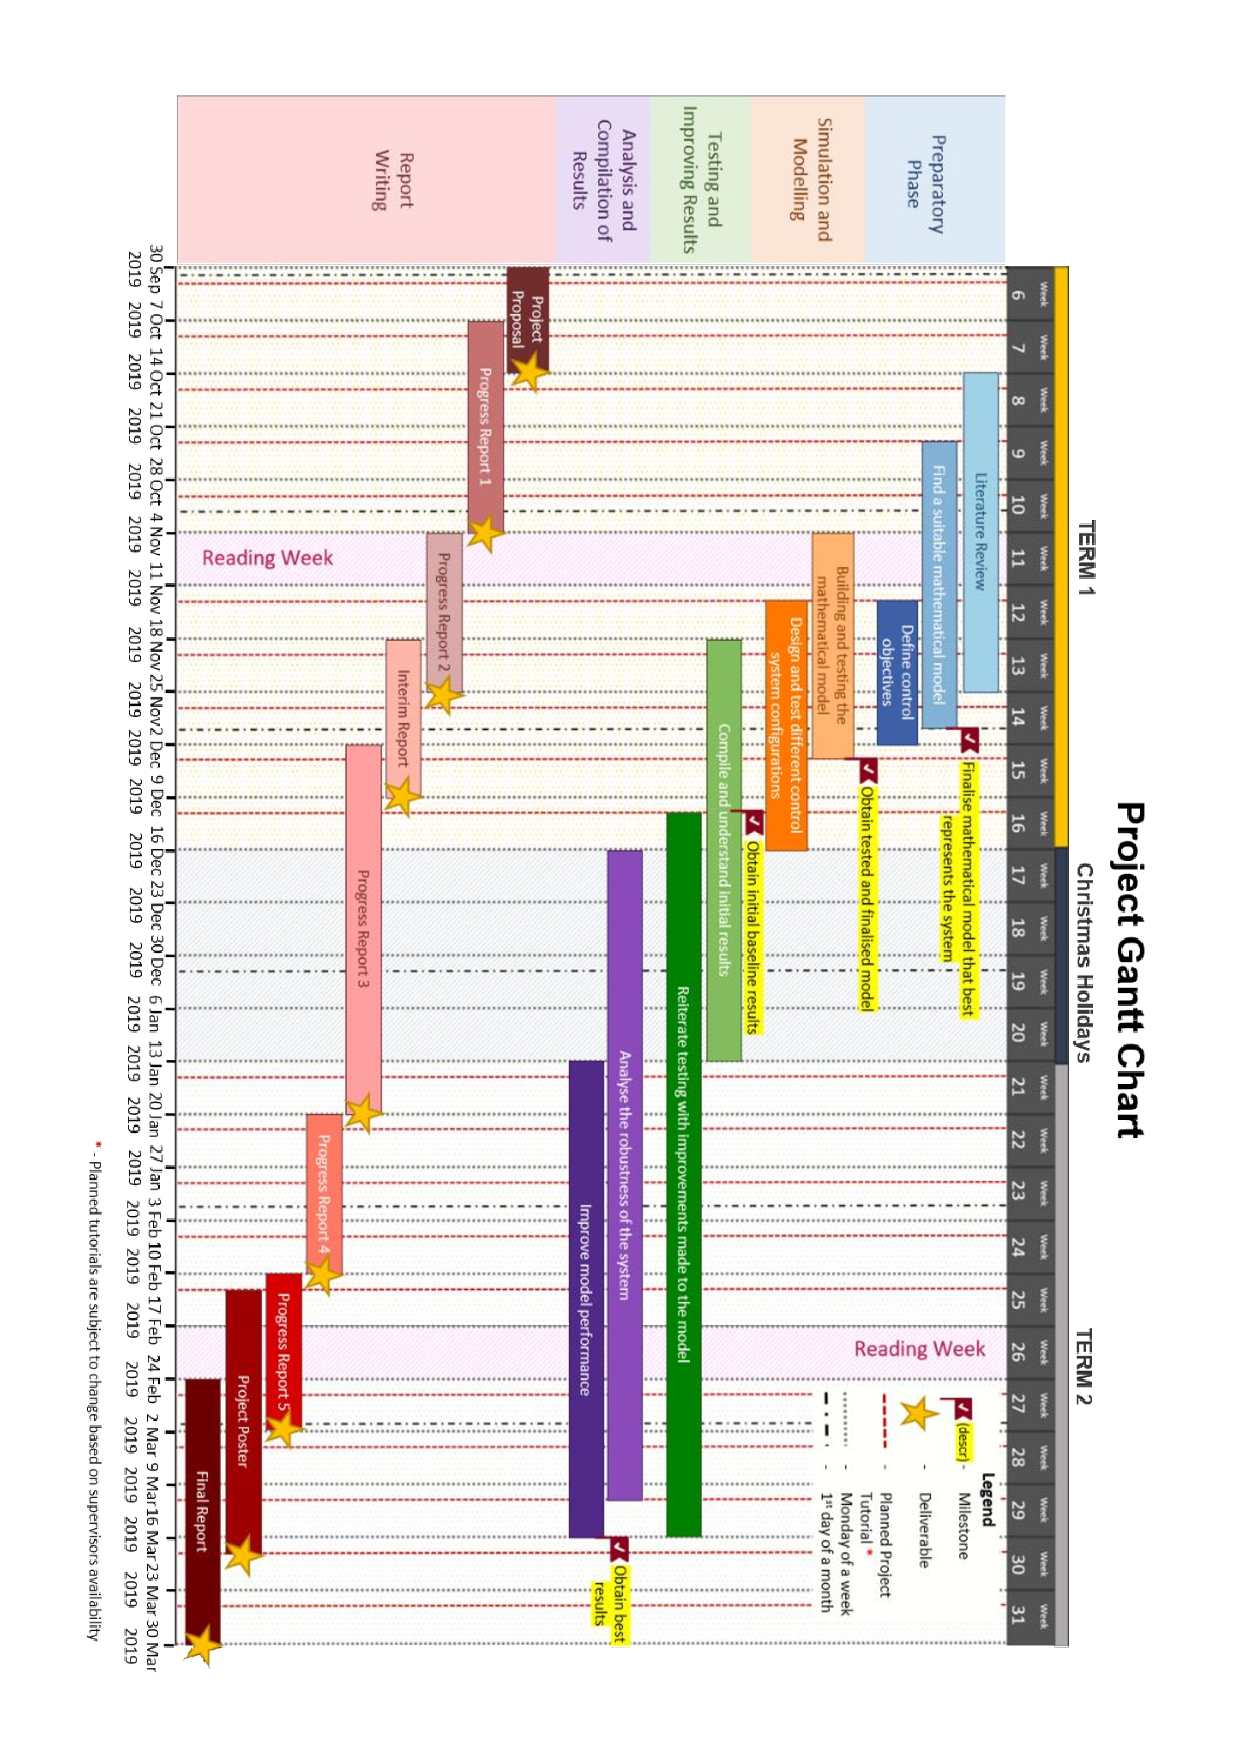
\includepdf[page=-]{files/Gantt Chart}
	\chapter{Risk Assessment}
	\label{appendix:b}
	The following hazards were identified through the risk assessment:
	\begin{itemize}
		\item Eyestrain
		\item Poor posture
		\item Repetitive movements involved with working on a computer
		\item Tripping over objects
		\item Poor lighting conditions
		\item Lone working
		\item Fire
		\item Contact with electricity
		\item General Welfare
	\end{itemize}
	The following pages includes a summary of the approved risk assessment generated using RiskNET.\\
	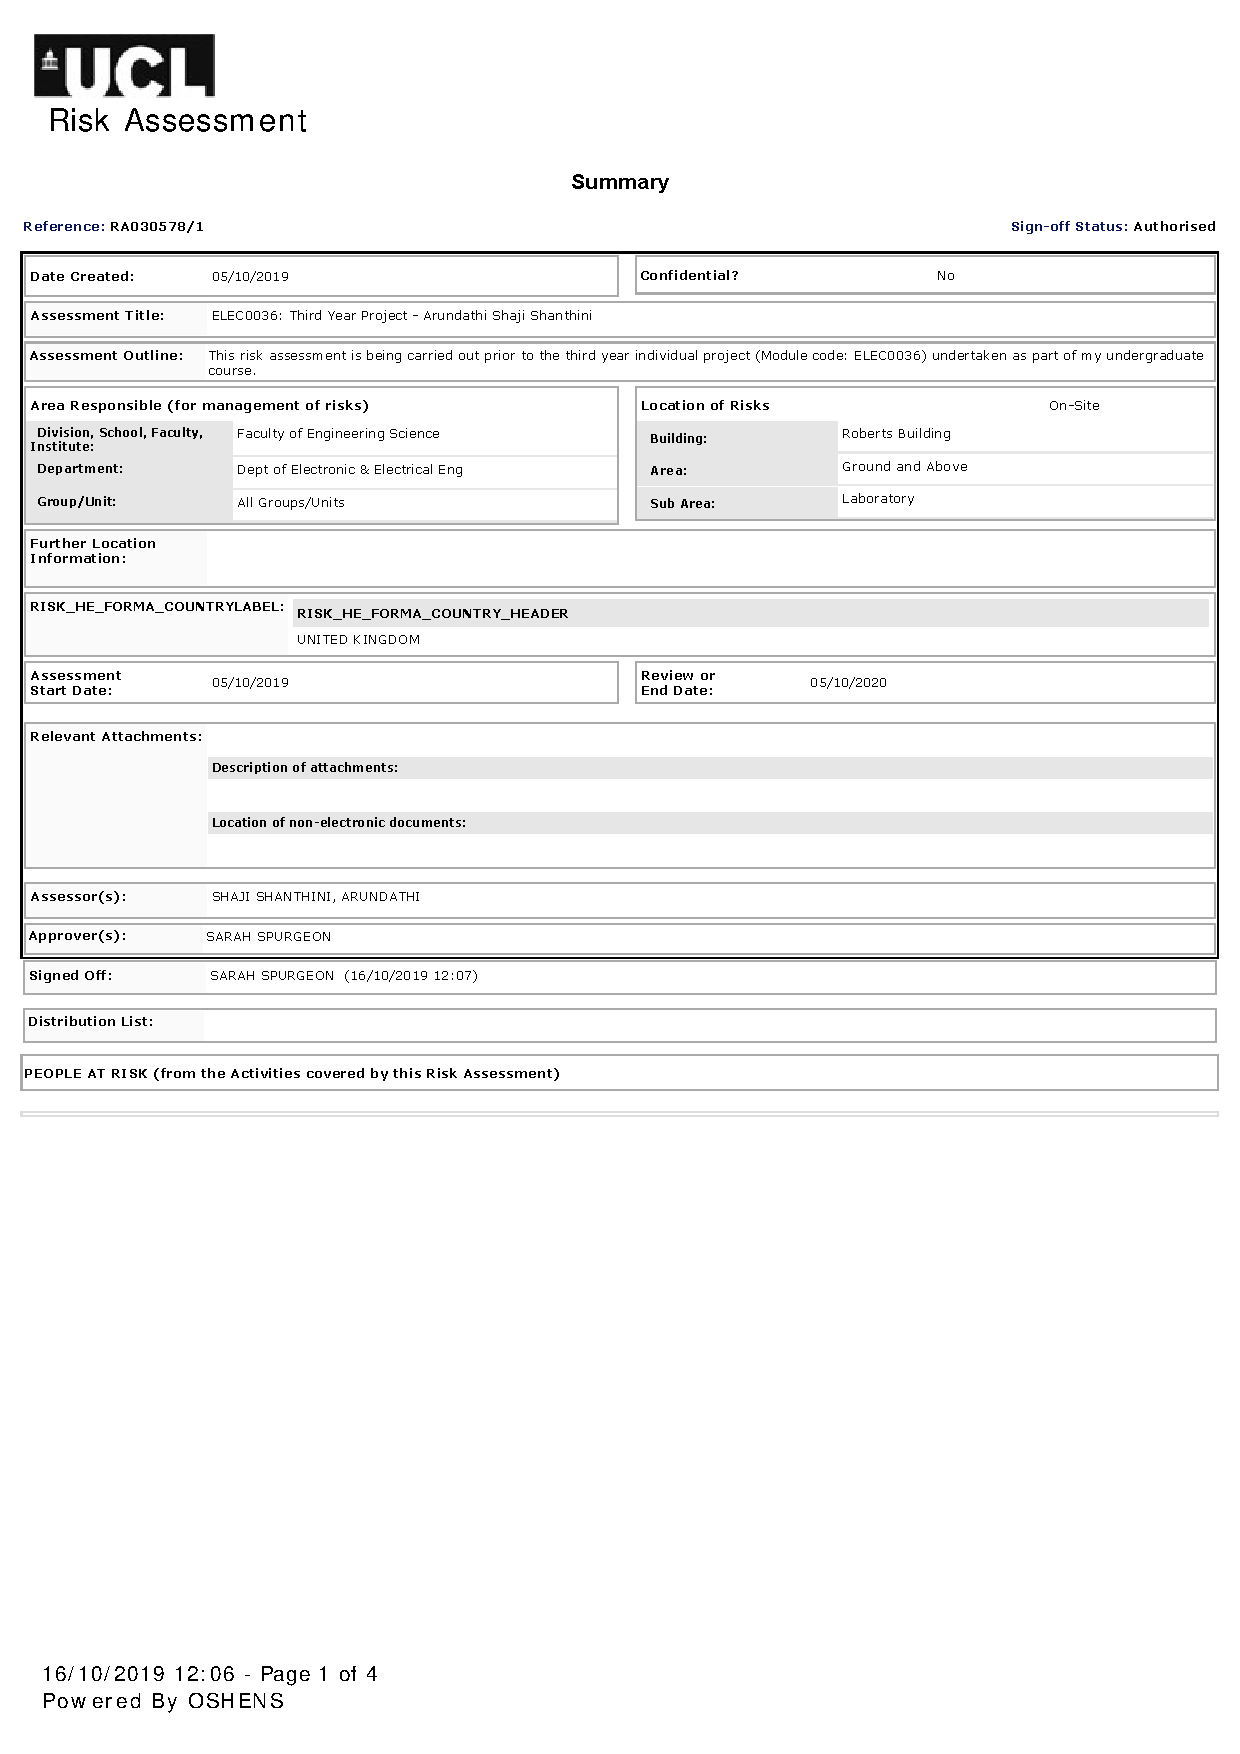
\includepdf[page=-]{files/Risk Assessment}
\end{appendices}
%%%%%%%%%%%%%%%%%%%%%%%%%%%%%%%%%%%%%%

\bibliographystyle{IEEEtran}
\bibliography{references}

\end{document}